\section{Applications of Neural Networks}
%Artificial neural networks have been around for a long time, since 1943 when in the paper, "A Logical Calculus of Ideas Immanent in Nervous Activity" McCulloch and Pitts presented a simplified computational model of how biological neurons might work together in animal brains to perform complex computations using propositional logic. The early successes of ANNs until the 1960s led to the widespread belief that we would soon be conversing with truly intelligent machines but the promise went unfulfilled. During the early 1980s there was some slow progress but in the 1990s more promising algorithms arrived, especially SVM. Only recently they have finally caught on due to the high volume of data available, increase of computing powers and especially GPU, better training algorithms and because some theoretical limitations, such as getting stuck in local minima, have turned out to rarely happen in practice.

%The mechanism of a biological neuron is very simple, but the network it belongs to is very complex. McCulloch and Walter Pitts proposed a very simple model of the biological neuron, which later became known as an artificial neuron: it has one or more binary (on/off) inputs and one binary output. The artificial neuron simply activates its output when more than a certain number of its inputs are active. McCulloch and Pitts showed that even with such a simplified model it is possible to build a network of artificial neurons that computes any logical proposition you want.

%The \tb{perceptron} is one of the simplest ANN architectures, invented in 1957 by Frank Rosenblatt. It is based on a slightly different artificial neuron called a threshold logic unit (TLU), or sometimes a linear threshold unit (LTU): the inputs and output are now numbers (instead of binary on/off values) and each input connection is associated with a weight, representing the importance of the input. The TLU computes a weighted sum of its inputs ($z = \sum_j w_j x_j = \x^T w)$, then applies a threshold to that sum. %and outputs the result: $hw(x) = step(z)$, where $z = \x^T w$. 
%\begin{equation}
%output \systeme*{0 \textit{ if } \sum_j w_j x_j \le \ti{threshold} ,1 \textit{ if } \sum_j w_j x_j> %\ti{threshold}}
%\end{equation}

%or equivalently
%\begin{equation}
%output \systeme*{0 \textit{ if } {\sum_j w_j x_j+b \le 0} ,1 \ti{ if } {\sum_j w_j x_j +b> 0}}
%\end{equation}

%You can think of the bias as a measure of how easy it is to get the perceptron to output a $1$. Or to put it in more biological terms, the bias is a measure of how easy it is to get the perceptron to fire. For a perceptron with a really big bias, it's extremely easy for the perceptron to output a 1. But if the bias is very negative, then it's difficult for the perceptron to output a 1

%Instead of thresholding, other common activation functions for the perceptron are \ti{Heavisde} or \ti{sign} functions:
%\begin{equation}
%\textit{heaviside} = \systeme*{0 \textit{ if } z<0,1 \textit{ if } z\ge 0}, \textit{sign} = \systeme*{-1 %\textit{ if } z<0,0 \textit{ if } z=0,1 \textit{ if } z>0}
%\end{equation}
%Also perceptrons, as they binary input ancestors, can be used is to compute the elementary logical functions we usually think of as underlying computation, functions such as AND, OR, and NAND.

%A single TLU can also be thought of as a simple linear binary classifier. If the result exceeds a threshold, it outputs the positive class or else outputs the negative class. A Perceptron is simply composed of a single layer of TLUs, with each TLU connected to all the inputs. 

%To see how learning might work, suppose we make a small change in some weight (or bias) in the network. What we'd like is for this small change in weight to cause only a small corresponding change in the output from the network. If it were true that a small change in a weight (or bias) causes only a small change in output, then we could use this fact to modify the weights and biases to get our network to behave more in the manner we want. And then we'd repeat this, changing the weights and biases over and over to produce better and better output. The network would be learning.

%The problem is that this isn't what happens when our network contains perceptrons. In fact, a small change in the weights or bias of any single perceptron in the network can sometimes cause the output of that perceptron to completely flip, say from 0 to 1. That flip may then cause the behaviour of the rest of the network to completely change in some very complicated way.

%We can overcome this problem by using a new type of artificial neuron using the \tb{sigmoid} function, instead of thresholding.  With sigmoid neurons, small changes in their weights and bias cause only a small change in their output, and the output can take any value between $0$ and $1$. Recall the sigmoid function:
%\begin{equation}
%\sigma = \frac{1}{1+e^{-\sum_j w_j x_j-b}}
%\end{equation}

%\subsection{Fully connected layers}
%When all the neurons in a layer are connected to every neuron in the previous layer (i.e., its input neurons), it is called a \tb{fully connected layer} or a \tb{dense layer}.

%In biology it is commonly said that \ti{cells that fire together, wire together}, meaning that the connection between two neurons gets stronger the one triggers often the other. For ANN, the connections is represented by weights and weights reinforces connection that reduce the error. The perceptrion is fed one training instance at a time: for each output neuron if its output is correct then it is ok at it is, if the prediction is wrong the weights from the inputs that would have contributed to the correct prediction must be reinforced.

%The outputs of a fully connected layer is $h_{w, b}(X) = \psi \br{XW+b}$. The weight update or learning rule is then:
%\begin{equation}
%w_{i,j}^{next} = w_{i,j} + \mu \br{y_j - \hat{y}_j}x_i
%\end{equation}
 
%The decision boundary of each output neuron is linear, so Perceptrons are incapable of learning complex patterns. However, if the training instances are separable, Rosenblatt demonstrated that this algorithm would converge to a solution (perceptron convergence theorem).
%In their 1969 monograph titled Perceptrons, Marvin Minsky and Seymour Papert highlighted a number of serious weaknesses of Perceptrons, in particular the fact that they are incapable of solving some trivial problems (e.g., the Exclusive OR (XOR) classification problem, such as any other linear classifier. However, by stacking multiple perceptrons (\ti{Multi-Layer Perceptron}) some of the limitations can be overcome. The inner layers of a MLP are called \tb{hidden layers}. The layers close to the input layer are usually called the lower layers, and the ones close to the outputs are usually called the upper layers. When a NN has many hidden layers, it is called a Deep Neural Network.

%\subsection{Backpropagation training algorithm}
%In 1986, David Rumelhart, Geoffrey Hinton and Ronald Williams published a groundbreaking paper introducing the backpropagation training algorithm, which is still used today. In short, it is simply Gradient Descent. 

%The algorithm consists of two steps, one forward and one backward. The algorithm handles one mini-batch at at time and each pass is called \ti{epoch}. For each mini-batch the algorithm computes the output of all neurons in a layer and pass it to the next layer, for every instance in the mini-batch (forward step). Then from the output layer the output error is measured. Then the algorithm measures how much each output connection contributed to the error by applying the chain rule. Then it measures how much error contributions  came from each connection in the previous layer and so on until the input layer (backward propagation). So now the error gradient across all connections is known. Finally the algorithm performs a Gradient Descent step to tweak all connection weights in the network using the error gradients it just computed.


%It is important to initialize all the hidden layers’ connection weights randomly, or else training will fail. For example, if you initialize all weights and biases to zero, then all neurons in a given layer will be perfectly identical, and thus backpropagation will affect them in exactly the same way, so they will remain identical. In other words, despite having hundreds of neurons per layer, your model will act as if it had only one neuron per layer: it won’t be too smart.

%To work properly the authors changed the step function of the MLP with the logistic function, since it is derivable everywhere. Two other popular activation function are:
%\begin{itemize}
%\item \textbf{hyprbolic tangent function} $\tanh(z) = 2\sigma(2z)-1$, whose values range from $-1$ to $1$. This tends to make each layer's output more or less centred around $0$ at the beginning of training speeding up the convergence.
%\item \textbf{Rectified Linear Unit function} $ReLU(z) = \max\br{0,z}$, which is continuous but not differentiable. In practice it works well and it is fast to compute.
%\end{itemize}

%\begin{figure}
%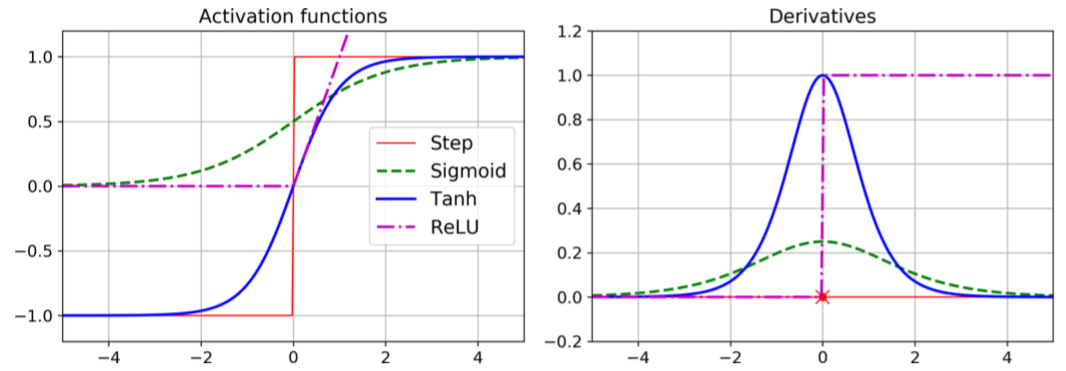
\includegraphics[scale=0.36]{img/activationFunctions}
%\caption{Shape of different activation functions.}
%\label{activationFunctions}
%\end{figure}


\subsection{MLP for regression tasks}
\tb{When building a MLP for regression one does not want to use any activation function for the output neurons} in order to let them take any possible value. To make it output only positive values, one can use the ReLU or \ti{softplus} activation functions. If a limited range of values is needed, one can use the \ti{logistic function} or \ti{hyperbolic tangent} and scale the labels to 0 and 1 for the logistic function or to -1 and 1 for the hyperbolic function.

The loss function is typically the MSE, if there are many outliers the mean absolute error is better, or the Huber which is a mix of the two.

\begin{figure}
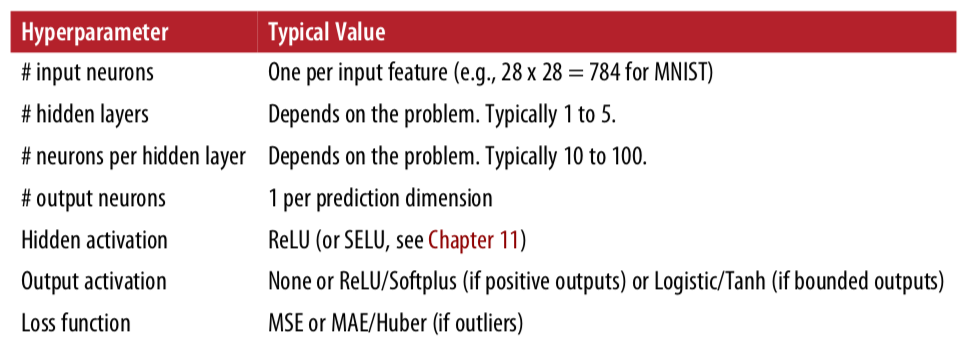
\includegraphics[scale=0.4]{img/NNRegArchitecture}
\caption{Common architecture for a regression NN.}
\end{figure}

\subsection{Classification MLP}
For a binary classification problem a single output neuron is needed using the logistic activation function. The output value will be in the range of $0$ and $1$ and will represent the probability. For multilabel binary classification tasks, two output neurons  both using the logistic activation function are needed (one neuron for each independent class). Instead if each instance can belong only to a single class out of 3 or more classes, one needs an output neuron per class using the softmax activation function for the whole output layer. The cross-entropy function is generally a good choice.

\begin{figure}
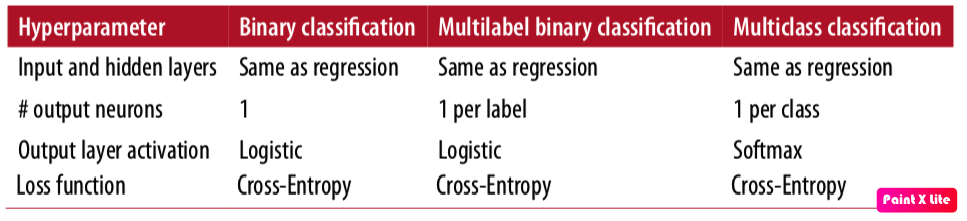
\includegraphics[scale=0.4]{img/NNClassArchitecture}
\caption{Common architecture for a classification NN.}
\end{figure}

\subsection{keras NN}
keras is a high-level Deep Learning API that allows to build, train and evaluate NN. The hard-work is done by a back-end that can be TensorFlow, Microsoft Congnitive Talk or Theano or even others. Tensorflow itself now comes with its own version of Keras (\ti{tf.keras}) which supports only TensorFlow as back-end but as some useful TensorFlow API.

\subsubsection{Training a sequential NN image classifier}
\begin{lstlisting}
import tensorflow as tf
from tensorflow import keras
fashion_mnist = keras.datasets.fashion_mnist
(X_train_full, y_train_full), (X_test, y_test) = 
					fashion_mnist.load_data()
 class_names = ["T-shirt/top", "Trouser", "Pullover", "Dress", "Coat", "Sandal", "Shirt", "Sneaker", "Bag", "Ankle boot"]
model = keras.models.Sequential()
model.add(keras.layers.Flatten(input_shape=[28, 28]))
model.add(keras.layers.Dense(300, activation="relu"))
model.add(keras.layers.Dense(100, activation="relu"))
model.add(keras.layers.Dense(10, activation="softmax"))
\end{lstlisting}

The first line creates a Sequential model. This is the simplest kind of Keras model, for neural networks that are just composed of a single stack of layers, connected sequentially. This is called the sequential API. Next, we build the first layer and add it to the model. It is a Flatten layer whose role is simply to convert each input image into a 1D array: if it receives input data $X$, it computes $X.reshape(-1, 1)$. This layer does not have any parameters, it is just there to do some simple preprocessing. Since it is the first layer in the model, you should specify the \lstinline+input_shape+: this does not include the batch size, only the shape of the instances. Alternatively, you could add a \lstinline+keras.layers.InputLayer+ as the first layer, setting \lstinline+shape=[28,28]+. Next we add a Dense hidden layer with 300 neurons. It will use the ReLU activation function. Each Dense layer manages its own weight matrix, containing all the connection weights between the neurons and their inputs. It also manages a vector of bias terms (one per neuron). Next we add a second Dense hidden layer with 100 neurons, also using the ReLU activation function. Finally, we add a Dense output layer with 10 neurons (one per class), using the softmax activation function (because the classes are exclusive).

Alternatively instead of adding each single layer, one can pass the list of layers to the constructor:
\begin{lstlisting}
model = keras.models.Sequential([keras.layers.Flatten(input_shape=[28, 28]), keras.layers.Dense(300, activation="relu"), keras.layers.Dense(100, activation="relu"), keras.layers.Dense(10, activation="softmax")])
model.layers[1].name #will return dense_3
model.get_layer("dense_3")
weights, biases = hidden1.get_weights()
model.compile(loss="sparse_categorical_crossentropy",  optimizer="sgd", metrics=["accuracy"])
history = model.fit(X_train, y_train, epochs=30,
    validation_data=(X_valid, y_valid))
pd.DataFrame(history.history).plot(figsize=(8, 5)) plt.grid(True)
plt.gca().set_ylim(0, 1) # set the vertical range to [0-1] plt.show()
\end{lstlisting}

\lstinline+summary+ method displays all the model's layers and their parameters.

Notice that the Dense layer initialized the connection weights randomly, and the biases were just initialized to zeros, which is fine.

To compile the model is crated, one must call \lstinline+compile+ method to specify the loss function and the optimizer to use.

This requires some explanation. First, we use the \lstinline+sparse_categorical+\lstinline+_crossentropy+ loss because we have sparse labels (i.e., for each instance there is just a target class index, from 0 to 9 in this case, i.e., 3 to represent class 3), and the classes are exclusive. If instead we had one target probability per class for each instance (such as one-hot vectors, e.g. \lstinline+[0., 0., 0., 1., 0., 0., 0., 0., 0., 0.]+ to represent class 3), then we would need to use the \lstinline+categorical_crossentropy+ loss instead. If we were doing binary classification (with one or more binary labels), then we would use the \lstinline+sigmoid+ (i.e., logistic) activation function in the output layer instead of the \lstinline+softmax+ activation function, and we would use the \lstinline+binary_crossentropy+ loss.

Secondly, regarding the optimizer, \lstinline+sgd+ simply means that we will train the model using simple Stochastic Gradient Descent.

To train the model one just need to call the $fit$ method, passing the training data, the number of epochs to train and optionally a validation set to measure the improvement at the end of each epoch and to avoid overfitting. Calling  $fit$ twice will result in continuing the training where it has been left from the first call.

If the training set was very skewed, with some classes being overrepresented and others underrepresented, it would be useful to set the \lstinline+class_weight+ argument when calling the \lstinline+fit()+ method, giving a larger weight to underrepresented classes, and a lower weight to overrepresented classes. These weights would be used by Keras when computing the loss. If you need per-instance weights instead, you can set the \lstinline+sample_weight+ argument (it supersedes \lstinline+class_weight+). This could be useful for example if some instances were labeled by experts while others were labeled using a crowdsourcing platform: you might want to give more weight to the former. You can also provide sample weights (but not class weights) for the validation set by adding them as a third item in the \lstinline+validation_data+ tuple.
Frame using this dictionary and call its plot() method, you get the learning curves shown.

If the model is not satisfactory, the hyper-paramaters must be adjusted. Only when it is satisfactory it can be evaluated on the test set using the \lstinline+evaluate()+ method. It is strictly forbidden to tweak the hyper-parameters on the test set because it will alter the generalization error.

To predict new data one just uses \lstinline+predict()+ method.

If you create a Pandas Data.......

\subsubsection{Training a sequential NN regressor}
Let us consider California housing problem again. The dataset will now contain only numerical features. The main difference from the NN classifier is that the output layer has a single neuron and uses no activation function, and the loss function is the MSE

\begin{lstlisting}
from sklearn.datasets import fetch_california_housing 
from sklearn.model_selection import train_test_split 
from sklearn.preprocessing import StandardScaler
    housing = fetch_california_housing()
    X_train_full, X_test, y_train_full, y_test = train_test_split(
        housing.data, housing.target)
    X_train, X_valid, y_train, y_valid = train_test_split(
        X_train_full, y_train_full)
    scaler = StandardScaler()
    X_train_scaled = scaler.fit_transform(X_train)
    X_valid_scaled = scaler.transform(X_valid)
    X_test_scaled = scaler.transform(X_test)
    
    model = keras.models.Sequential([
        keras.layers.Dense(30, activation="relu", input_shape=X_train.shape[1:]),
        keras.layers.Dense(1)
    ])
    model.compile(loss="mean_squared_error", optimizer="sgd")
    history = model.fit(X_train, y_train, epochs=20,
                        validation_data=(X_valid, y_valid))
    mse_test = model.evaluate(X_test, y_test)
X_new = X_test[:3] # pretend these are new instances y_pred = model.predict(X_new)
\end{lstlisting}

\subsubsection{Non sequential model}
One example of a non-sequential neural network is a Wide \& Deep neural network. This neural network architecture was introduced in a 2016 paper by Heng-Tze Cheng et al.14. It connects all or part of the inputs directly to the output layer. This architecture makes it possible for the neural network to learn both deep patterns (using the deep path) and simple rules (through the short path). In contrast, a regular MLP forces all the data to flow through the full stack of layers, thus simple patterns in the data may end up being distorted by this sequence of transformations.

\begin{lstlisting}
input = keras.layers.Input(shape=X_train.shape[1:])
hidden1 = keras.layers.Dense(30, activation="relu")(input)
hidden2 = keras.layers.Dense(30, activation="relu")(hidden1)
concat = keras.layers.Concatenate()([input, hidden2])
output = keras.layers.Dense(1)(concat)
model = keras.models.Model(inputs=[input], outputs=[output])
\end{lstlisting}

First, we need to create an Input object. This is needed because we may have multiple inputs, as we will see later. Next, we create a dense layer with 30 neurons and using the ReLU activation function. As soon as it is created, notice that we call it like a function, passing it the input. This is why this is called the Functional API. We are telling Keras how it should link layers together. We then create a second hidden layer, and again we use it as a function. Note however that we pass it the output of the first hidden layer. Next, we create a \lstinline+Concatenate()+ layer, and once again we immediately use it like a function, to concatenate the input and the output of the second hidden layer (you may prefer the \lstinline+keras.layers.concatenate()+ function, which creates a \lstinline+Concatenate+ layer and immediately calls it with the given inputs). 

Then we create the output layer, with a single neuron and no activation function, and we call it like a function, passing it the result of the concatenation. Lastly, we create a Keras Model, specifying which inputs and outputs to use.

Suppose now that there are 8 features and we want to send a subset of features (from 2 to 7) through the long path and a possibly overlapping subset feature (from 0 to 4) to the output layer:
\begin{lstlisting}
input_A = keras.layers.Input(shape=[5])
input_B = keras.layers.Input(shape=[6])
hidden1 = keras.layers.Dense(30, activation="relu")(input_B)
hidden2 = keras.layers.Dense(30, activation="relu")(hidden1)
concat = keras.layers.concatenate([input_A, hidden2])
output = keras.layers.Dense(1)(concat)
model = keras.models.Model(inputs=[input_A, input_B], outputs=[output])
model.compile(loss="mse", optimizer="sgd")
    X_train_A, X_train_B = X_train[:, :5], X_train[:, 2:]
    X_valid_A, X_valid_B = X_valid[:, :5], X_valid[:, 2:]
    X_test_A, X_test_B = X_test[:, :5], X_test[:, 2:]
    X_new_A, X_new_B = X_test_A[:3], X_test_B[:3]
    history = model.fit((X_train_A, X_train_B), y_train, epochs=20, validation_data=((X_valid_A, X_valid_B), y_valid))
    mse_test = model.evaluate((X_test_A, X_test_B), y_test)
    y_pred = model.predict((X_new_A, X_new_B))
output = keras.layers.Dense(1)(concat)
aux_output = keras.layers.Dense(1)(hidden2)
model = keras.models.Model(inputs=[input_A, input_B], outputs=[output, aux_output])
\end{lstlisting}
We must pass also different labels:
\begin{lstlisting}
history = model.fit(
        [X_train_A, X_train_B], [y_train, y_train], epochs=20,
        validation_data=([X_valid_A, X_valid_B], [y_valid, y_valid]))
\end{lstlisting}

Now when calling the \lstinline+fit+ method one must pass the two input matrices $A$ and $B$.

Each output will need its own loss function, so when we compile the model we should pass a list of losses (if we pass a single loss, Keras will assume that the same loss must be used for all outputs). By default, Keras will compute all these losses and simply add them up to get the final loss used for training. However, if we care much more about the one output, so we give the main output's loss a much greater weight. Fortunately, it is possible to set all the loss weights when compiling the model:
\begin{lstlisting}
model.compile(loss=["mse", "mse"], loss_weights=[0.9, 0.1], optimizer="sgd")
\end{lstlisting}
				
Non sequential NNs may be required for example when we want to locate and classify the main object in a picture: this is both a regression and classification task. Another example is when having multiple independent task on the same data: this gives a better result than training one neural network per task.

\subsubsection{Dyanamic models}
Both sequential and non-sequential models presented are static. Sometimes it is good to have dynamic behaviours. For such cases the Subclass API is helpful. Simply subclass the Model class, create the layers you need in the constructor, and use them to perform the computations you want in the \lstinline+call()+ method. For example, creating an instance of the following WideAndDeepModel class gives us an equivalent model to the one we just built with the Functional API. You can then compile it, evaluate it and use it to make predictions, exactly like already did.

\begin{lstlisting}
class WideAndDeepModel(keras.models.Model):
    def __init__(self, units=30, activation="relu", **kwargs):
        super().__init__(**kwargs) # handles standard args (e.g., name) self.hidden1 = keras.layers.Dense(units, activation=activation) self.hidden2 = keras.layers.Dense(units, activation=activation) self.main_output = keras.layers.Dense(1)
        self.aux_output = keras.layers.Dense(1)

    def call(self, inputs):
         input_A, input_B = inputs
         hidden1 = self.hidden1(input_B)
         hidden2 = self.hidden2(hidden1)
         concat = keras.layers.concatenate([input_A, hidden2]) main_output = self.main_output(concat)
         aux_output = self.aux_output(hidden2)
         return main_output, aux_output

model = WideAndDeepModel()
\end{lstlisting}
The \lstinline+call+ method allows extra flexibility granting the possibility to introduce loops, conditional statements and low level TensorFlow operations. However, this extra flexibility comes at a cost: your model’s architecture is hidden within the \lstinline+call()+ method, so Keras cannot easily inspect it, it cannot save or clone it, and when you call the \lstinline+summary()+ method, you only get a list of layers, without any information on how they are connected to each other. Moreover, Keras cannot check types and shapes ahead of time, and it is easier to make mistakes. So unless you really need that extra flexibility, you should probably stick to the Sequential API or the Functional API.

\subsubsection{Saving and restoring the model}
To save and load the model:
\begin{lstlisting}
model.save("my_keras_model.h5");
....
model = keras.models.load_model("my_keras_model.h5")
\end{lstlisting}
Keras will save both the architecture and the values of all the parameters. When the training is tool long, it is better to save the model at regular steps during the run of the fit method with callbacks.

\subsubsection{Callbacks to save the model during fit}
The \lstinline+fit()+ method accepts a callbacks argument that lets you specify a list of objects that Keras will call during training at the start and end of training, at the start and end of each epoch and even before and after processing each batch. For example, the \lstinline+ModelCheckpoint+ callback saves checkpoints of your model at regular intervals during training, by default at the end of each epoch:
\begin{lstlisting}
checkpoint_cb = keras.callbacks.ModelCheckpoint("my_keras_model.h5")
history = model.fit(X_train, y_train, epochs=10, callbacks=[checkpoint_cb])
\end{lstlisting}

Moreover, if you use a validation set during training, you can set \lstinline+save_best_only=True+ when creating the ModelCheckpoint. In this case, it will only save your model when its performance on the validation set is the best so far. This is a simple way to implement early stopping:
\begin{lstlisting}
checkpoint_cb = keras.callbacks.ModelCheckpoint("my_keras_model.h5", save_best_only=True)
history = model.fit(X_train, y_train, epochs=10, validation_data=(X_valid, y_valid), callbacks=[checkpoint_cb])
model = keras.models.load_model("my_keras_model.h5") # rollback to best model
\end{lstlisting}

Another way to implement early stopping is to simply use the \cd+EarlyStopping+ callback. It will interrupt training when it measures no progress on the validation set for a number of epochs (defined by the \cd+patience+ argument), and it will optionally roll back to the best model. You can combine both callbacks to both save checkpoints of your model (in case your computer crashes), and actually interrupt training early when there is no more progress (to avoid wasting time and resources):

\begin{lstlisting}
early_stopping_cb = keras.callbacks.EarlyStopping(patience=10, restore_best_weights=True)
history = model.fit(X_train, y_train, epochs=100, validation_data=(X_valid, y_valid), callbacks=[checkpoint_cb, early_stopping_cb])
\end{lstlisting}
The number of epochs can be set to a large value since training will stop automatically when there is no more progress. Moreover, there is no need to restore the best model saved in this case since the EarlyStopping callback will keep track of the best weights and restore them for us at the end of training.

One can also write custom callbacks:
\begin{lstlisting}
class PrintValTrainRatioCallback(keras.callbacks.Callback): 
    def on_epoch_end(self, epoch, logs):
        print("\nval/train: {:.2f}".format(logs["val_loss"] 
        			/ logs["loss"]))
\end{lstlisting}

As you might expect, you can implement \lstinline+on_train_begin()+, \lstinline+on_train_end()+, \lstinline+on_epoch_begin()+, \lstinline+on_epoch_begin()+, \lstinline+on_batch_end()+ and \lstinline+on_batch_end()+. Moreover, callbacks can also be used during evaluation and predictions, should you ever need them (e.g., for debugging). In this case, you should implement \lstinline+on_test_begin()+, \lstinline+on_test_end()+, \lstinline+on_test_batch_begin()+, or \lstinline+on_test+\lstinline+_batch+\lstinline+_end()+ (called by \lstinline+evaluate()+), or \lstinline+on_predict_begin()+, \lstinline+on_predict_end()+, \lstinline+on_+\lstinline+predict+\lstinline+_batch_begin()+, or \lstinline+on_predict_batch+\lstinline+_end()+ (called by \lstinline+predict()+).

\subsubsection{Tensorboard}
TensorBoard is a great interactive visualization tool that you can use to view the learning curves during training, compare learning curves between multiple runs, visualize the computation graph, analyze training statistics, view images generated by your model, visualize complex multidimensional data projected down to 3D and automatically clustered for you, and more! This tool is installed automatically when you install TensorFlow, so you already have it!

To use it, you must modify your program so that it outputs the data you want to visualize to special binary log files called event files. Each binary data record is called a summary.

Let us start by defining the root log directory we will use for our TensorBoard logs, plus a small function that will generate a subdirectory path based on the current date and time, so that it is different at every run. You may want to include extra information in the log directory name, such as hyperparameter values that you are testing, to make it easier to know what you are looking at in TensorBoard:

\begin{lstlisting}
root_logdir = os.path.join(os.curdir, "my_logs")

def get_run_logdir(): import time
    run_id = time.strftime("run_%Y_%m_%d-%H_%M_%S")
    return os.path.join(root_logdir, run_id)
run_logdir = get_run_logdir() # e.g., './my_logs/run_2019_01_16-11_28_43'
\end{lstlisting}

Next, the good news is that Keras provides a nice \lstinline+TensorBoard+ callback:

\begin{lstlisting}
tensorboard_cb = keras.callbacks.TensorBoard(run_logdir) history = model.fit(X_train, y_train, epochs=30,
	validation_data=(X_valid, y_valid),
    callbacks=[tensorboard_cb])
\end{lstlisting}

Next you need to start the TensorBoard server. If you installed TensorFlow within a virtualenv, you should activate it. Next, run the following command at the root of the project. Then run \lstinline+tensorboard --logdir=./my_logs --port=6006+.
\subsection{Fine tuning a NN}
One way is to tune the many hyperparameters is try different combinations and check which works better in the validation set. For this approach one can use \lstinline+GridSearchCV+ or \lstinline+RandomizedSearchCV+.
\begin{lstlisting}
def build_model(n_hidden=1, n_neurons=30, learning_rate=3e-3, input_shape=[8]): 
    model = keras.models.Sequential()
    options = {"input_shape": input_shape}
    for layer in range(n_hidden):
        model.add(keras.layers.Dense(n_neurons, activation="relu", **options))
        options = {} 
    model.add(keras.layers.Dense(1, **options)) optimizer = keras.optimizers.SGD(learning_rate)         
    model.compile(loss="mse", optimizer=optimizer) 
    return model
    
keras_reg = keras.wrappers.scikit_learn.KerasRegressor(build_model)
\end{lstlisting}
This function creates a simple Sequential model. The options \lstinline+dict+ is used to ensure that the first layer is properly given the input shape. The \lstinline+KerasRegressor+ object is a thin wrapper around the Keras model built using \lstinline+build_model()+.

\begin{lstlisting}
keras_reg.fit(X_train, y_train, epochs=100,
		validation_data=(X_valid, y_valid),
    		callbacks=[keras.callbacks.EarlyStopping(patience=10)])
mse_test = keras_reg.score(X_test, y_test)
y_pred = keras_reg.predict(X_new)
\end{lstlisting}

Note that the score will be the opposite of the MSE because Scikit-Learn wants scores, not losses. However, we want to train hundreds of variants and see which one performs best on the validation set. Since there are many hyperparameters, it is preferable to use a randomized search rather than grid search.
Let's try to explore the number of hidden layers, the number of neurons and the learning rate

\begin{lstlisting}
from scipy.stats import reciprocal
from sklearn.model_selection import RandomizedSearchCV
param_distribs = {
        "n_hidden": [0, 1, 2, 3],
        "n_neurons": np.arange(1, 100),
        "learning_rate": reciprocal(3e-4, 3e-2),
}
rnd_search_cv = RandomizedSearchCV(keras_reg, param_distribs, n_iter=10, cv=3)
rnd_search_cv.fit(X_train, y_train, epochs=100,
    validation_data=(X_valid, y_valid),
    callbacks=[keras.callbacks.EarlyStopping(patience=10)])
\end{lstlisting}
The exploration may last many hours depending on the hardware, the size of the dataset, the complexity of the model and the value of iterations and crossvalidations. When it is over, you can access the best parameters found, the best score, and the trained Keras model like this:

\begin{lstlisting}
>>> rnd_search_cv.best_params_
{'learning_rate': 0.0033625641252688094, 'n_hidden': 2, 'n_neurons': 42}
 >>> rnd_search_cv.best_score_
-0.3189529188278931
>>> model = rnd_search_cv.best_estimator_.model
\end{lstlisting}

However, when training is slow (e.g., for more complex problems with larger datasets), this approach will only explore a tiny portion of the hyperparameter space. You can partially alleviate this problem by assisting the search process manually: first run a quick random search using wide ranges of hyperparameter values, then run another search using smaller ranges of values centred on the best ones found during the first run, and so on. This will hopefully zoom in to a good set of hyperparameters. However, this is very time consuming, and probably not the best use of your time.

Fortunately, there are many techniques to explore a search space much more efficiently than randomly. Their core idea is simple: when a region of the space turns out to be good, it should be explored more. There are many Python libraries to do this "zooming process".

\subsubsection{Number of hidden layers}
For many problems a single hidden layer is enough. However \tb{deep networks have a much higher parameter efficiency than shallow ones: they can model complex functions using exponentially fewer neurons than shallow nets, allowing them to reach much better performance with the same amount of training data}.

Real-world data is often structured in such a hierarchical way and Deep Neural Networks automatically take advantage of this fact: \tb{lower hidden layers model low-level structures (e.g., line segments of various shapes and orientations), intermediate hidden layers combine these low-level structures to model intermediate-level structures (e.g., squares, circles), and the highest hidden layers and the output layer combine these intermediate structures to model high-level structures (e.g., faces)}.

\tb{Not only does this hierarchical architecture help DNNs converge faster to a good solution, it also improves their ability to generalize to new datasets}. For example, if you have already trained a model to recognize faces in pictures, and you now want to train a new neural network to recognize hairstyles, then you can kickstart training by reusing the lower layers of the first network. Instead of randomly initializing the weights and biases of the first few layers of the new neural network, you can initialize them to the value of the weights and biases of the lower layers of the first network. This way the network will not have to learn from scratch all the low-level structures that occur in most pictures; it will only have to learn the higher-level structures (e.g., hairstyles). This is called \tb{transfer learning}.

In summary for many problems you can start with just one or two hidden layers and it will work just fine. For more complex problems, you can gradually ramp up the number of hidden layers, until you start overfitting the training set. Very complex tasks, such as large image classification or speech recognition, typically require networks with dozens of layers).

\subsubsection{Number of neurons per hidden layers}
It used to be a common practice to size them to form a pyramid, with fewer and fewer neurons at each layer the rationale being that many low-level features can coalesce into far fewer high-level features. However, this practice has been largely abandoned now, as it seems that simply \tb{using the same number of neurons in all hidden layers performs just as well in most cases, or even better, and there is just one hyperparameter to tune} instead of one per layer, for example, all hidden layers could simply have 150 neurons. However, depending on the dataset, it can sometimes help to make the first hidden layer bigger than the others.

Just like for the number of layers, you can try increasing the number of neurons gradually until the network starts overfitting. In general you will get more bang for the buck by increasing the number of layers than the number of neurons per layer. Unfortunately, as you can see, finding the perfect amount of neurons is still somewhat of a dark art.

A simpler approach is to pick a model with more layers and neurons than you actually need, then use early stopping to prevent it from overfitting (and other regularization techniques, such as dropout). This has been dubbed the "stretch pants" approach: instead of wasting time looking for pants that perfectly match your size, just use large stretch pants that will shrink down to the right size.


\subsubsection{Learning Rate, Batch Size and Other Hyperparameters}
\begin{itemize}
\item The \tb{learning rate} is arguably the most important hyperparameter. In general, the optimal learning rate is about half of the maximum learning rate (i.e., the learning rate above which the training algorithm diverges). So a simple approach for tuning the learning rate is to start with a large value that makes the training algorithm diverge, then divide this value by $3$ and try again, and repeat until the training algorithm stops diverging. At that point, you generally won't be too far from the optimal learning rate. That said, it is sometimes useful to reduce the learning rate during training.

\item Choosing a better optimizer than plain old Mini-batch Gradient Descent (and tuning its hyperparameters) is also quite important.
\item The \tb{batch size} can also have a significant impact on your model's performance and the training time. In general the optimal batch size will be lower than 32 (April 2018, Yann Lecun even tweeted "Friends don't let friends use mini-batches larger than 32"). A small batch size ensures that each training iteration is very fast, and although a large batch size will give a more precise estimate of the gradients, in practice this does not matter much since the optimization landscape is quite complex and the direction of the true gradients do not point precisely in the direction of the optimum. However, having a batch size greater than 10 helps take advantage of hardware and software optimizations, in particular for matrix multiplications, so it will speed up training. Moreover, if you use Batch Normalization, the batch size should not be too small (in general no less than 20).
\item In most cases, the number of training iterations does not actually need to be tweaked: just use early stopping instead.
\end{itemize}